% Circumscribed Parallelepiped
% Author: Axel Pavillet
\documentclass[tikz,border=10pt]{standalone}
%%%<
\usepackage{verbatim}
\usepackage{amsmath, amssymb}
\usepackage{stmaryrd}
\usepackage{graphicx, subfigure}
\usepackage{color}
\usepackage[all]{xy}
\usepackage{extarrows}
\usepackage{proof}
\usepackage{hyperref}
\usepackage{wrapfig}
\usepackage{multirow}

\begin{document}
	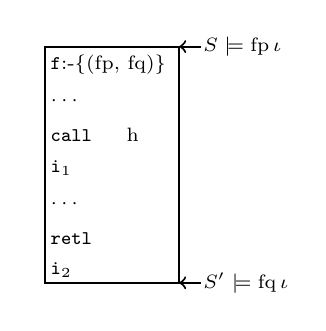
\begin{tikzpicture}[font=\scriptsize, line width=0.75pt]
		\draw[-] (0,0) rectangle (1.7, 3);
		\node(fun) at (0.8, 1.46)
		{
			$
			\begin{array}{l}
				\texttt{f} \text{:-\{(fp, fq)\}} \\
				\\[-3pt]
				\cdots \\
				\\[-3pt]
				\texttt{call} \quad \; \; \text{h} \\
				\\[-5pt]
				\texttt{i}_1 \\
				\\[-3pt]
				\cdots \\
				\\[-3pt]
				\texttt{retl} \\
				\\[-5pt]
				\texttt{i}_2
			\end{array}
			$
		};
		\node[right = 5pt] (pre) at (1.7, 3) {$S\models \text{fp} \, \iota$};
		\draw[->] (1.97, 3) -- (1.7, 3);
		\node[right = 5pt] (post) at (1.7, 0) {$S' \models \text{fq} \, \iota$};
		\draw[->] (1.97, 0) -- (1.7, 0);
	\end{tikzpicture}
\end{document}